\subsection{Section 4.2.2-Style Effectiveness Evaluation}

The following figures reproduce the effectiveness-evaluation style of Section 4.2.2 using the ArduPilot SITL dataset and the final V9/p99\_abs/W10\_N3\_mean1x recovery configuration.

\begin{figure*}[t]
    \centering
    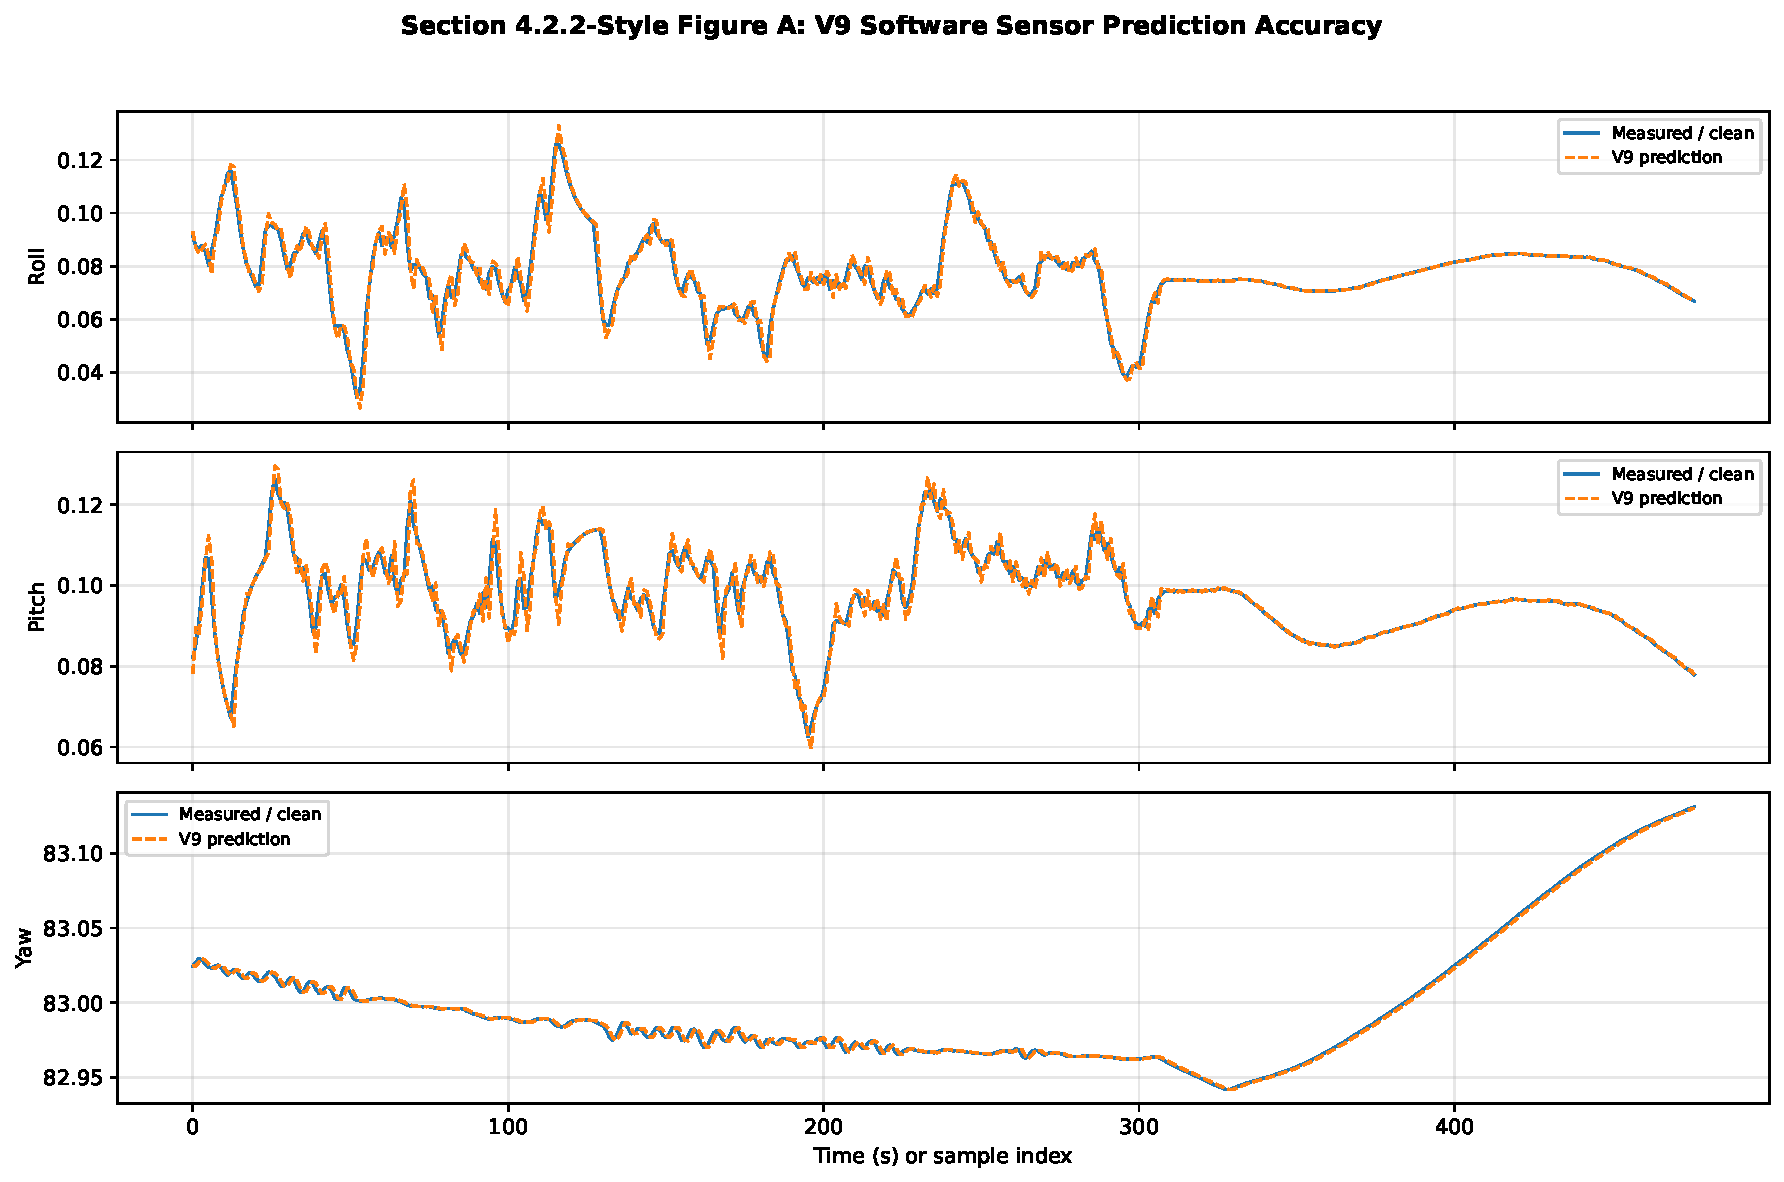
\includegraphics[width=0.95\textwidth]{phase7_section_4_2_2_effectiveness_figures/figure_4_2_2_a_v9_prediction_accuracy.pdf}
    \caption{V9 software-sensor prediction accuracy under clean or representative logs. The V9 predictor estimates the future attitude state using information available at time $k$.}
    \label{fig:v9_prediction_accuracy}
\end{figure*}

\begin{figure*}[t]
    \centering
    \includegraphics[width=0.95\textwidth]{phase7_section_4_2_2_effectiveness_figures/figure_4_2_2_b_clean_residual_threshold.pdf}
    \caption{Clean residual behavior and $p99\_abs$ threshold. The threshold is estimated from clean residuals and later used to identify abnormal deviations under attack.}
    \label{fig:clean_residual_threshold}
\end{figure*}

\begin{figure*}[t]
    \centering
    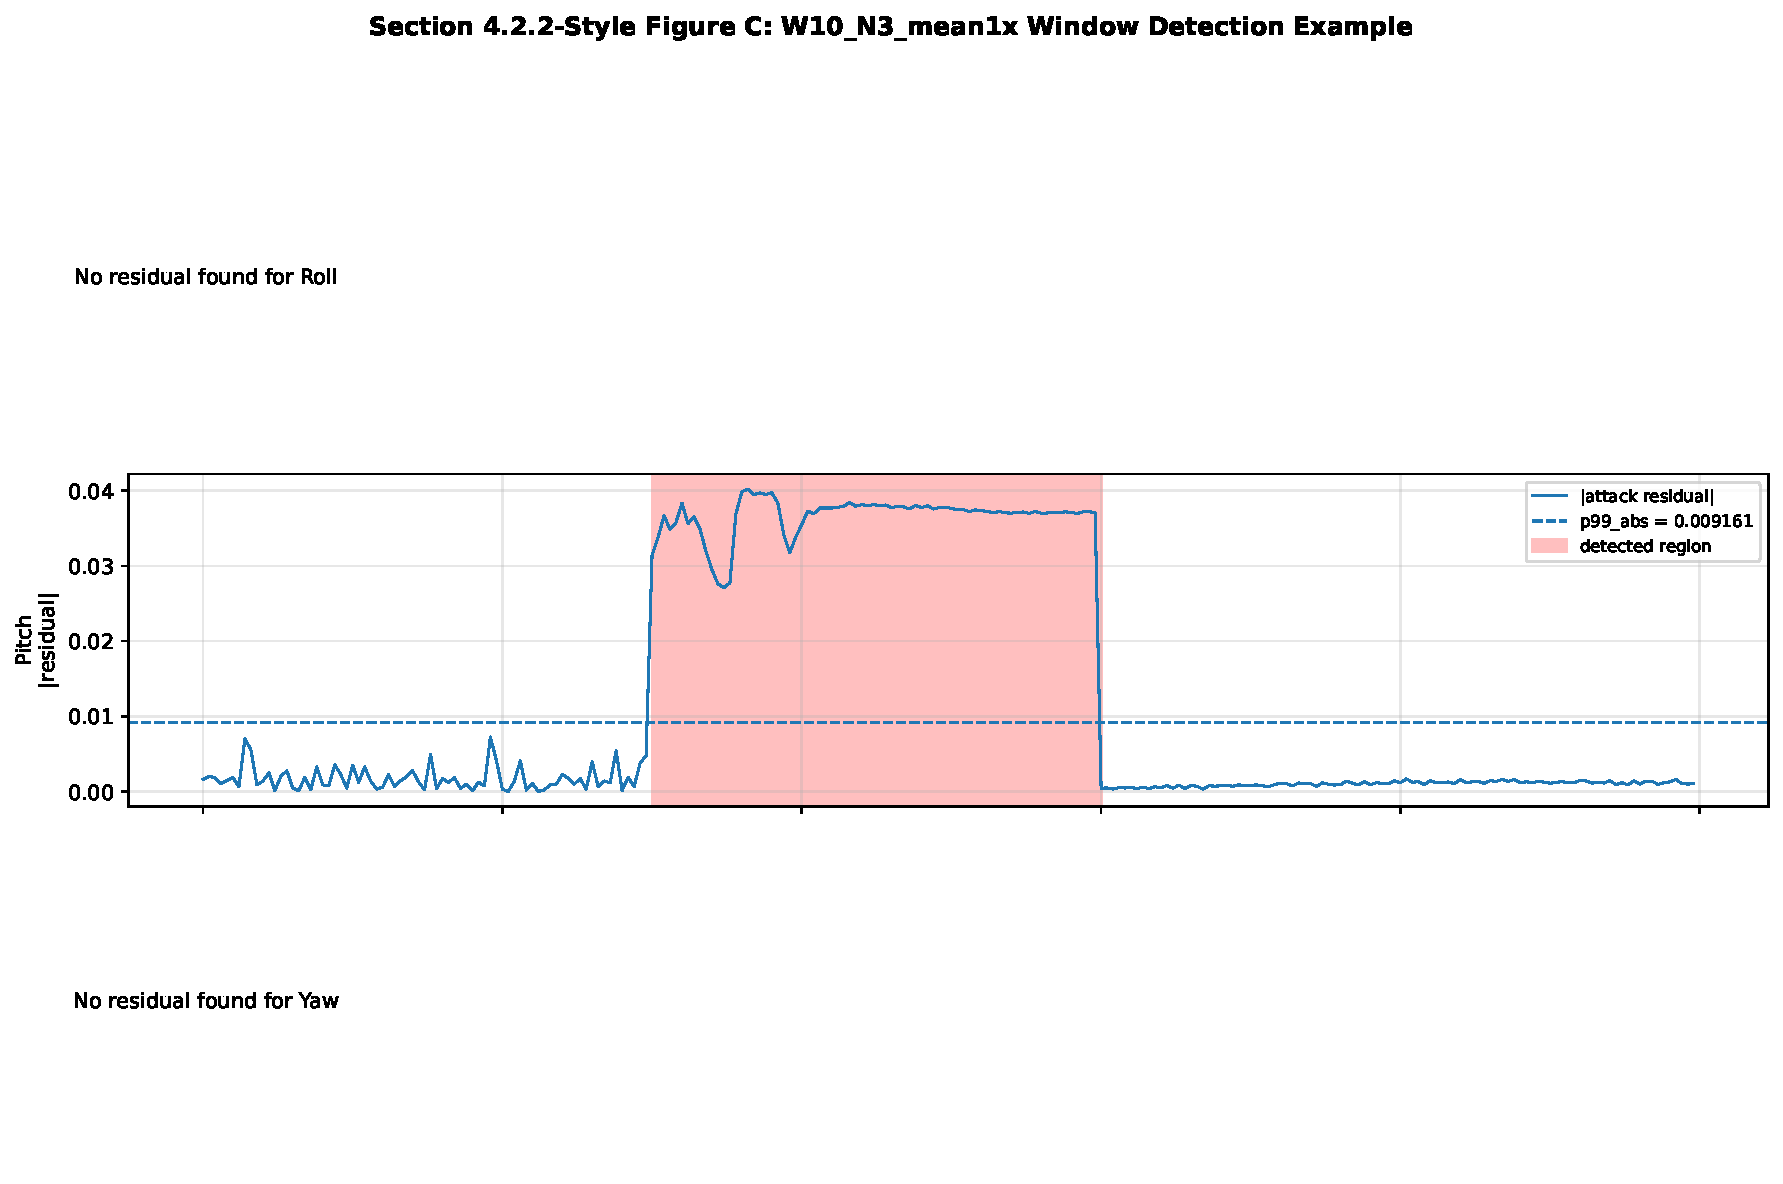
\includegraphics[width=0.95\textwidth]{phase7_section_4_2_2_effectiveness_figures/figure_4_2_2_c_window_detection_example.pdf}
    \caption{Window-based detection using W10\_N3\_mean1x. The detector declares an attack when at least three threshold violations occur inside a ten-sample window.}
    \label{fig:window_detection_example}
\end{figure*}

\begin{figure*}[t]
    \centering
    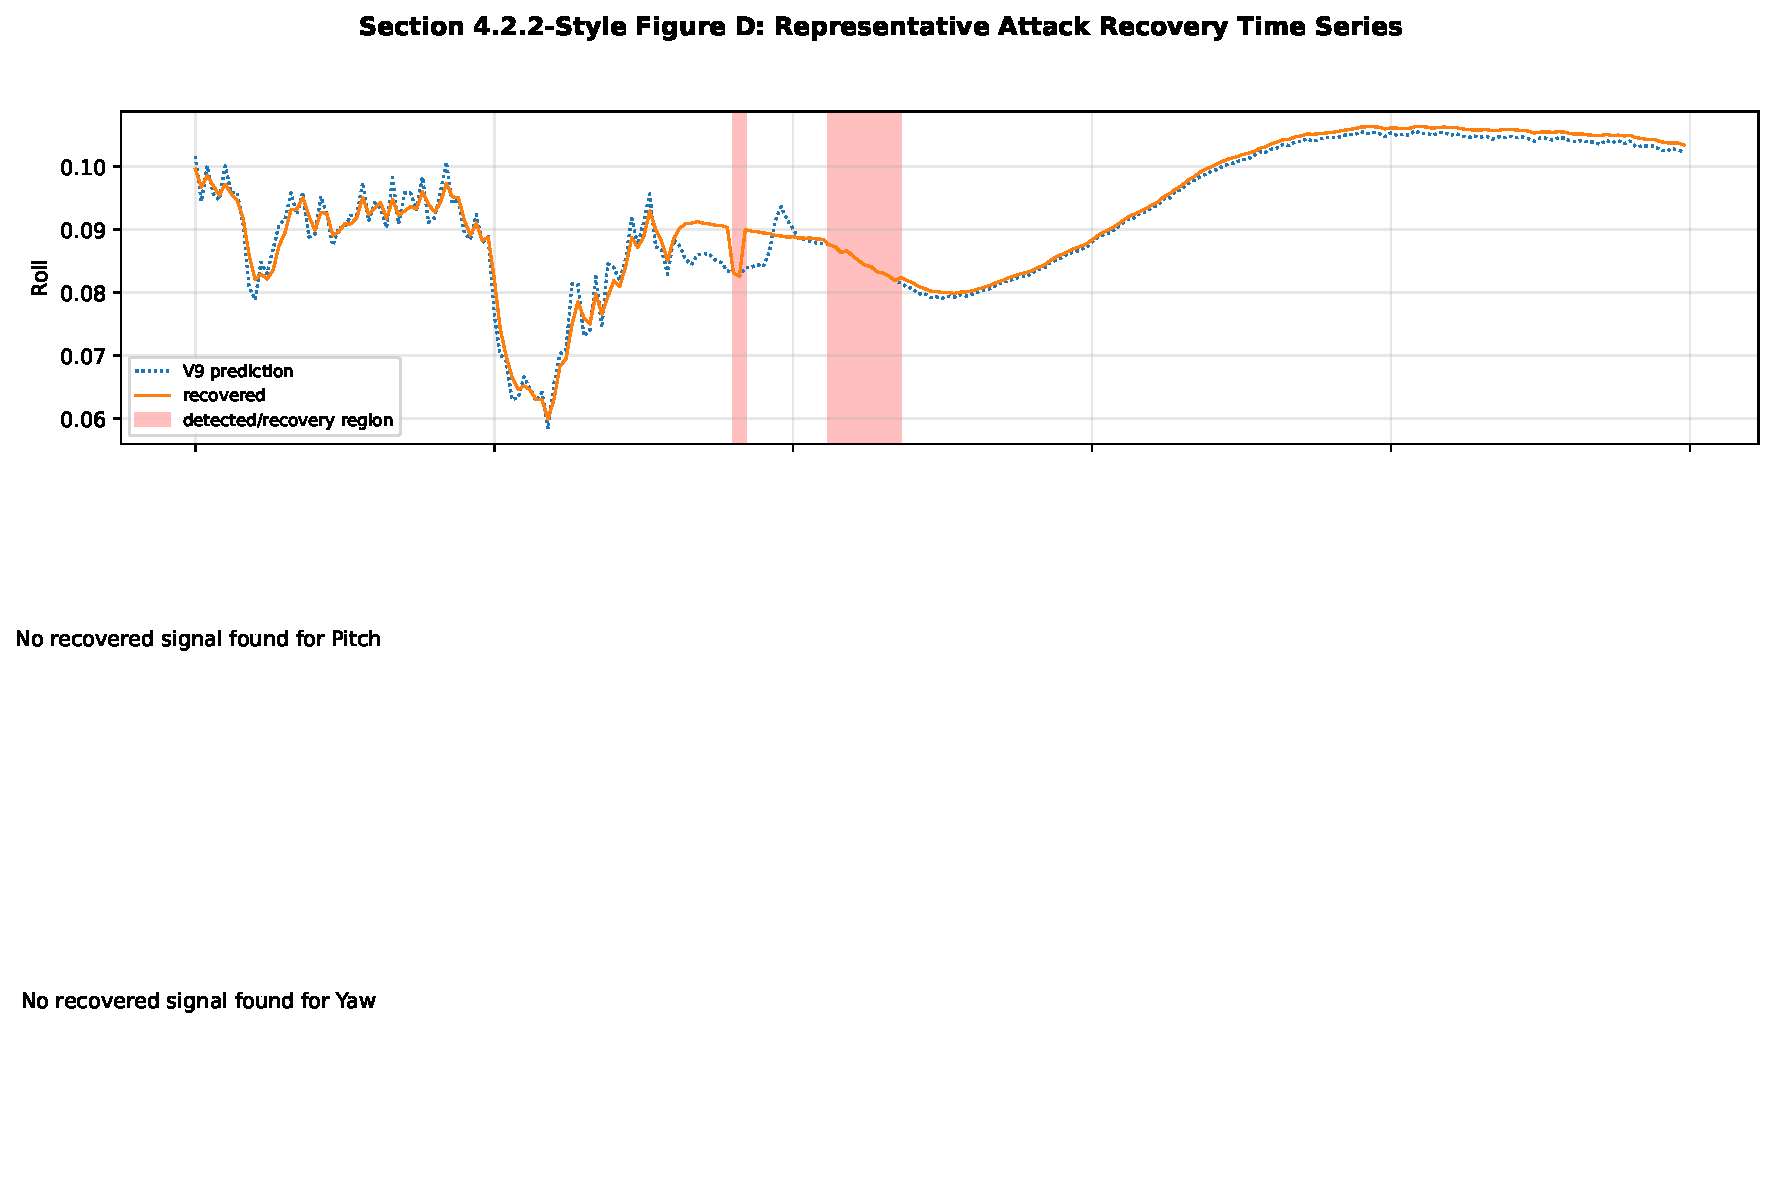
\includegraphics[width=0.95\textwidth]{phase7_section_4_2_2_effectiveness_figures/figure_4_2_2_d_recovery_timeseries_example.pdf}
    \caption{Representative attack recovery time series. During detected attack periods, the corrupted measurement is replaced by the V9 software-sensor prediction.}
    \label{fig:recovery_timeseries_example}
\end{figure*}

\begin{figure}[t]
    \centering
    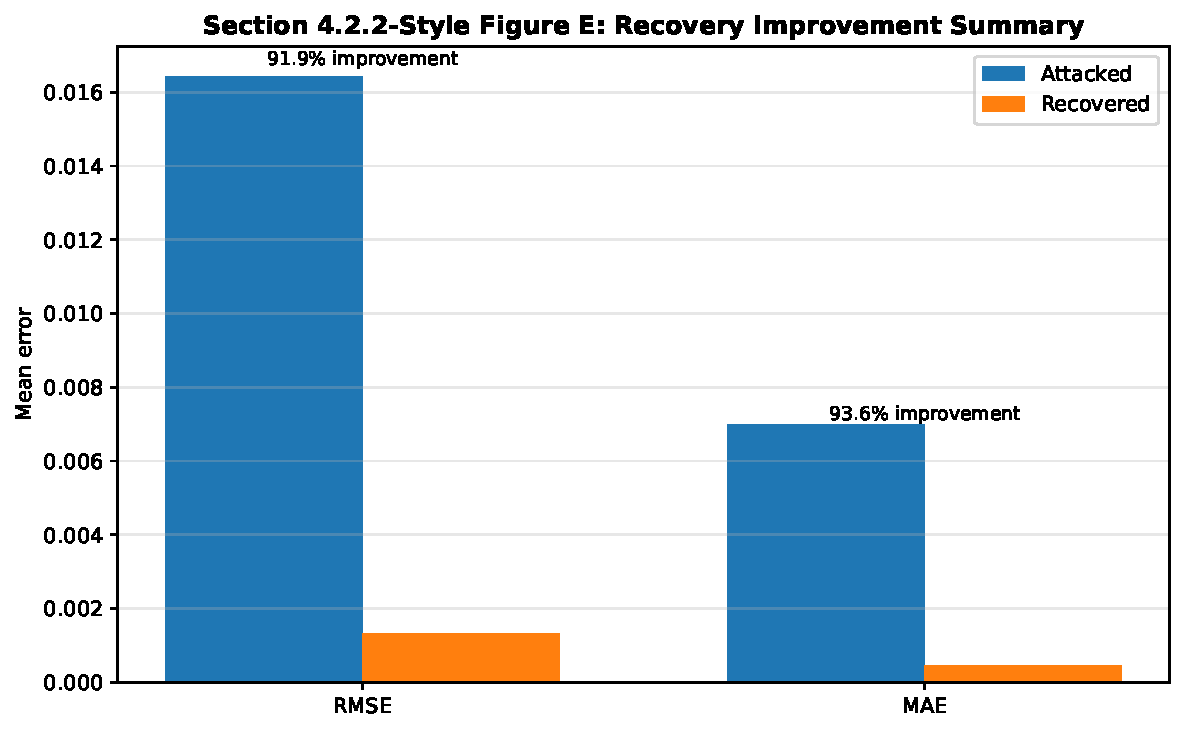
\includegraphics[width=0.48\textwidth]{phase7_section_4_2_2_effectiveness_figures/figure_4_2_2_e_recovery_improvement_summary.pdf}
    \caption{Mean recovery improvement summary. The recovered signal reduces RMSE and MAE compared with the attacked measurement.}
    \label{fig:recovery_improvement_summary}
\end{figure}
